% !TeX spellcheck = en_US

\documentclass[a4paper, oneside, 12pt]{report}

% ----------- packages -------------

\usepackage[a4paper,width=150mm,top=25mm,bottom=25mm]{geometry}

\usepackage[utf8]{inputenc}
\usepackage[english]{babel}
\usepackage[T1]{fontenc}
\usepackage{lmodern}

\usepackage{graphicx}
\graphicspath{{images/}}

\usepackage{amsmath}
\usepackage{amsthm}
\usepackage{amssymb}
\usepackage{wasysym}

\usepackage{algorithm}
\usepackage[noend]{algpseudocode}

\usepackage{setspace}

\usepackage{hyperref}

\usepackage[dvipsnames]{xcolor}

\bibliographystyle{plainurl}

% ----------- macros -------------

\newtheorem{theorem}{Theorem}
\newtheorem{corollary}{Corollary}
\newtheorem{lemma}{Lemma}
\newtheorem{proposition}{Proposition}

\theoremstyle{definition}
\newtheorem{definition}{Definition}

\theoremstyle{remark}
\newtheorem*{remark}{Remark}

\algdef{SE}[DOWHILE]{Do}{doWhile}{\algorithmicdo}[1]{\algorithmicwhile\ #1}%

\newcommand{\MinAlg}{\textsc{MinimizeDFA}}
\newcommand{\CompUnr}{\textsc{ComUnreachables}}
\newcommand{\RemUnr}{\textsc{RemUnreachables}}
\newcommand{\CompDist}{\textsc{ComEquivPairs}}
\newcommand{\RemEq}{\textsc{RemEquivPairs}}
\newcommand{\mmD}{\mathcal{D}}

\newcommand{\gregorColor}{Violet}
\newcommand{\gregor}[1]{\textcolor{\gregorColor}{\textbf{Gregor:} #1}}

% ----------- content -------------

\title{Generation of DFA Minimization Problems}
\author{Gregor Hans Christian Sönnichsen}

\begin{document}
	
	\maketitle
	
	\begin{abstract}
		Abstract$\ldots$
	\end{abstract}

	\renewcommand{\abstractname}{Generierung von DFA Minimierungsproblemen\\-\\Zusammenfassung}
	\begin{abstract}
		Zusammenfassung$\ldots$
	\end{abstract}
	
	%\chapter*{Acknowledgements}
	%I want to thank...
	
	\renewcommand{\contentsname}{Table of Contents}
	\tableofcontents
	
	% !TeX spellcheck = en_US

\chapter{Introduction}

% study computer science, (theoretical informatics), automata theory, value of this theory

Automata theory is recommended as part of a standard computer science curriculum~\cite[pp. 5-6]{GI16}. As other such theories it provides the chance to gain a precise cognitive model yielding new perspectives on problems and givens. This may thus lead to increased problem solving skills and more accurate thinking.

% typical topic - minimization, (why typical)

A typical task in automata theory is the minimization of a given deterministic finite automaton (DFA). The classic textbook ``Introduction to automata theory, languages, and computation'' by Hopcroft et. al.~\cite{HMU01} presents a practicable minimization algorithm. In this work we will confine ourselves to look at DFA minimizations using that algorithm.

% sketch situation

In an introduction course to theoretical computer science minimization tasks are thus likely to occur in supplementary exercises or exams. As of the creation of such tasks, one may assume, that it is done mostly manually. Automation would yield here the following advantages:

\begin{itemize}
	\item freeing time for other things, e.g. research, helping students face-to-face, designing the whole exercise sheet
	
	\item generation of tasks which lie in a well-defined range
	
	\item increased predictability and consistency of the generated task properties, which can be adjusted accurately through various parameters
	
	\item saves human operators from the generating task which involves monotonous work
\end{itemize}
\gregor{Delete or find extern from wikipedia}
Engagement on this topic promises moreover increased clarification which kind of minimization tasks can be generated, and where difficulties of those tasks lie.

This work aims to provide theoretical foundations for a DFA minimization task generator. What requirements a user has towards such a program will be discussed in a short requirements analysis. Based on this work a DFA minimization generator has been implemented. It can be found at \url{https://github.com/bt701607/Generation-of-DFA-Minimization-Problems}.

\section{Preliminaries}

We start with defining preliminary theoretical foundations.

\subsection{Deterministic Finite Automatons}

A 5-tuple $A = (Q, \Sigma, \delta, s, F)$ with $Q$ being a finite set of \emph{states}, $\Sigma$ a finite set of \emph{alphabet symbols}, $\delta \colon\ Q \times \Sigma \to Q$ a \emph{transition function}, $s \in Q$ a \emph{start state} and $F \subseteq Q$ \emph{final states} is called \emph{deterministic finite automaton} (DFA)~\cite[p. 46]{HMU01}. From now on $\mathfrak{A}$ shall denote the set of all DFAs.

We say $\delta(q,\sigma) = p$ is a transition from $q$ to $p$ using symbol $\sigma$. We define the \emph{extended transition function} $\delta^* : Q \times \Sigma^* \to Q$ of a DFA $A = (Q, \Sigma, \delta, s, F)$ as:
\begin{itemize}
	\item $\delta^*(q,\varepsilon) = q$
	\item $\delta^*(q,w\sigma) = \delta(\delta^*(q,w),\sigma)$ for all $q \in Q$, $w \in \Sigma^*$, $\sigma \in \Sigma$
\end{itemize}
Then, the \emph{language} of that DFA is defined as $L(A) = \{\ w\ |\ \delta^*(w) \in F\ \}$~\cite[pp. 49-50. 52]{HMU01}.

Given a state $q \in Q$. With $d^-(q)$ we denote the set of all \emph{ingoing} transitions $\delta(q', \sigma) = q$ of $q$. With $d^+(q)$ we denote the set of all \emph{outgoing} transitions $\delta(q, \sigma) = q'$ of $q$~\cite[pp. 2-3]{CP05}. If a transition is of the form $\delta(q, \sigma) = q$, then we say that $q$ has a \emph{loop}.

\begin{definition}\label{ch:1:unreachable-states}
	We say a state $q$ is \emph{(un-)reachable} in a DFA $A$, iff there is (no) a word $w \in \Sigma^*$ such that $\delta^*(s, w) = q$.
\end{definition}
\noindent If all states of a DFA $A$ are reachable, then we say $A$ is \emph{accessible}~\cite[p. 2]{CP05}.

A DFA is called \emph{complete} iff for all states, every symbol of the alphabet is used on an outgoing transition: $\forall q\in Q\colon \forall\sigma\in\Sigma\colon \exists p\in Q\colon \delta(q,\sigma) = p$. Note, that every incomplete DFA can be converted to a complete one by adding a so called \emph{dead state}~\cite[p. 67]{HMU01}. The resulting automaton has the same language.

\begin{figure}
	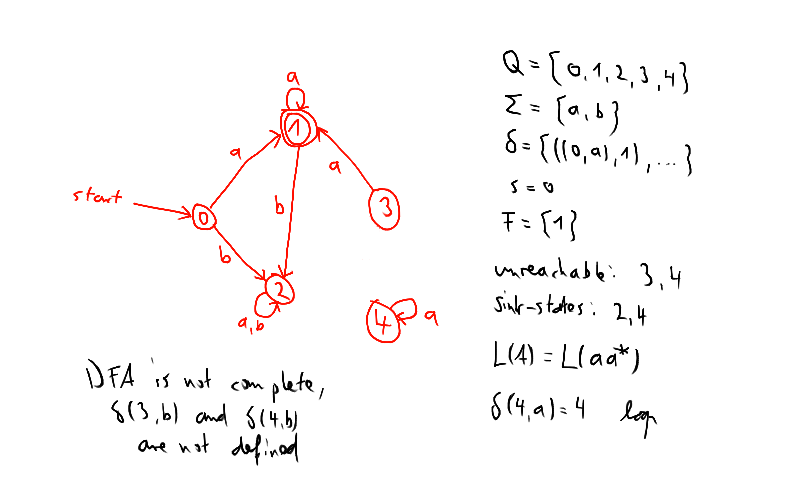
\includegraphics[width=\linewidth]{images/dfa.png}
	\caption{An example DFA and its properties.}
	\label{fig:dfa}
\end{figure}

\subsection{Minimal DFAs}

This section closely follows~\cite[pp. 42-45]{Sch01}. We call a DFA $A$ \emph{minimal}, if there exists no other automaton with the same language using less states. With $\mathfrak{A}_{min}$ we shall denote the set of all minimal DFAs.

The \emph{Nerode-relation} $\equiv_L\ \subseteq\ \Sigma^* \times \Sigma^*$ of a language $L$ with alphabet $\Sigma$ is defined as follows:
\begin{displaymath}
	x \equiv_L y\ \Leftrightarrow_{def}\ \forall z\in\Sigma^*\colon (xz\in L \Leftrightarrow yz\in L)
\end{displaymath}
The Nerode-relation of a DFA $A$ is the the Nerode-relation of its language: $\equiv_{L(A)}$. If the context makes it clear, than we will shorten the notation of a equivalence class $[x]_{\equiv_L}$ with $[x]$.

The \emph{equivalence class automaton} $A_L = (Q_L, \Sigma_L, \delta_L, s_L, F_L)$ to a regular language $L$ with alphabet $\Sigma$ is defined as follows:
\begin{itemize}
	\item $Q_L = \{\ [x]\ |\ x \in \Sigma^*\ \}$
	\item $\Sigma_L = \Sigma$
	\item $\delta_L([x], \sigma) = [x\sigma],\ \forall x\in\Sigma^*,\ \forall\sigma\in\Sigma$
	\item $s = [\varepsilon]$
	\item $F = \{\ [x]\ |\ x \in L\ \}$
\end{itemize}
\begin{theorem}
	Given a language $L$, then the equivalence class automaton $A_L$ is minimal.
\end{theorem}

\subsection{Practical Isomorphy of DFAs}

Given two DFAs $A_1 = (Q_1, \Sigma_1, \delta_1, s_1, F_1)$ and $A_2 = (Q_2, \Sigma_2, \delta_2, s_2, F_2)$. We say $A_1$ and $A_2$ are \emph{practical isomorph}, iff:
\begin{itemize}
	\item $|Q_1| = |Q_2|$, $|\Sigma_1| = |\Sigma_2|$ and
	\item there exists a bijection $\phi\colon \Sigma_1 \to \Sigma_2$ such that:
	\item there exists a bijection $\pi\colon Q_1 \to Q_2$ such that:
	
	$\pi(s_1) = s_2$
	
	$\forall q\in Q_1\colon (q\in F_1 \Longleftrightarrow \pi(q)\in F_2)$
	
	$\forall q\in Q_1\colon \forall\sigma\in\Sigma_1\colon \pi(\delta_1(q,\sigma))=\delta_2(\pi(q),\phi(\sigma)))$
\end{itemize}
Note that practical isomorphy between two DFAs $A_1, A_2$ does not imply $L(A_1) = L(A_2)$. This would be given, if $\Sigma_1 = \Sigma_2$ were the case (see~\cite[p. 45]{Sch01}). However the language of such DFAs is equivalent except for an exchange of alphabet symbols:
\[
	\{\ \phi(\sigma_0)\ldots\phi(\sigma_n)\ |\ \sigma_0\ldots\sigma_n\in L(A_1)\ \} = L(A_2)
\]
Practical isomorphy will be sufficient for our case. \gregor{why?}
%\begin{theorem} \textnormal{\cite[p. 45]{Sch01}} 
%	Every minimal DFA is unique except for isomorphy.
%\end{theorem}
%So it
%\begin{corollary}\label{ch:1:cor:all-min-dfa-ism}
%	Every minimal DFA $A$ is isomorph to its corresponding equivalence class automaton $A_{L(A)}$.
%	\gregor{All min. DFAs are ism. to each other, including A\_L}
%\end{corollary}
\gregor{Write down isomorphism test. Maybe discuss faster methods here? Look for faster methods in general?}

\subsection{Equivalent and distinguishable state pairs}

\begin{definition}[Equivalent and Distinguishable State Pairs]\cite[p. 154]{HMU01}
	A state pair $q_1, q_2 \in Q$ of a DFA $A = (Q, \Sigma, \delta, s, F)$ is called \emph{equivalent}, iff $\sim_A(q_1, q_2)$ is true, whereas
	\begin{displaymath}
	q_1\ \sim_A\ q_2 \Leftrightarrow_{def}\ \forall z \in \Sigma^* \colon\ (\delta^*(q_1, z) \in F \Leftrightarrow \delta^*(q_2, z) \in F)
	\end{displaymath}
	If $q_0 \not\sim_A q_1$, then $q_0$ and $q_1$ are called a \emph{distinguishable} state pair. The relation $\sim_A$ is an equivalence relation
\end{definition}
%\noindent Note the similarity between $\equiv_{L(A)}$ and $\sim_A$.:
%\begin{align*}
%	x\ \equiv_{L(A)}\ y\ \Leftrightarrow&\ \forall z\in\Sigma^*\colon (xz \in L \Leftrightarrow yz \in L) \\
%	& \\
%	q_1\ \sim_A\ q_2\ \Leftrightarrow&\ \forall z \in \Sigma^* \colon\ (\delta^*(q_1, z) \in F \Leftrightarrow \delta^*(q_2, z) \in F)
%\end{align*}
%We will prove the following statement regarding both relations:
%\begin{proposition}[Relationship of $\equiv_{L(A)}$ and $\sim_A$] \label{ch:1:prop-ner-eq} $ $ \\
%    \[
%    	x \equiv_{L(A)} y\ \Leftrightarrow\ \delta^*(s,x)=q_1\ \land\ \delta^*(s,y)=q_2\ \land\ q_1 \sim_A q_2
%    \]
%\end{proposition}
%\noindent Informally said: $x \equiv_{L(A)} y$ is true if and only if $q_1 \sim_A q_2$ whereas $q_1, q_2$ are reachable via $x,y$.
%\begin{proof} Via direct proof.
%    \begin{align*}
%    \ \delta^*(s,x)=q_1 \land \delta^*(s,y)=q_2\ \land\ & q_1 \sim_A q_2 \\
%    \Leftrightarrow\ \delta^*(s,x)=q_1 \land \delta^*(s,y)=q_2\ \land\ &(\forall z \in \Sigma^* \colon\ \delta^*(q_1, z) \in F \Leftrightarrow \delta^*(q_2, z) \in F) \\
%    \Leftrightarrow\hspace{5.65cm}&\ \forall z \in \Sigma^* \colon\ \delta^*(\delta^*(s,x), z) \in F \Leftrightarrow \delta^*(\delta^*(s,y), z) \in F \\
%    \Leftrightarrow\hspace{5.65cm}&\ \forall z \in \Sigma^* \colon\ \delta^*(s,xz) \in F \Leftrightarrow \delta^*(s,yz) \in F \\
%    \Leftrightarrow\hspace{5.65cm}&\ \forall z \in \Sigma^* \colon\ xz \in L(A) \Leftrightarrow yz \in L(A) \\
%    \Leftrightarrow\hspace{5.65cm}& x \equiv_{L(A)} y
%    \end{align*}
%\end{proof}
%\begin{corollary}
%    If the DFA $A$ is accessible, then there exists a $1:1$-correspondence between the equivalence classes of $\equiv_{L(A)}$ and $\sim_A$.
%\end{corollary}

%\noindent Proposition~\ref{ch:1:prop-ner-eq} can be supplemented by an even stronger declaration. Towards this declaration we first define, analogous to the equivalence class automaton, the \emph{$\sim$-equivalence automaton} $A_{\sim_A} = (Q_{\sim_A}, \Sigma_{\sim_A}, \delta_{\sim_A}, s_{\sim_A}, F_{\sim_A})$ to a DFA $A$:
%\begin{itemize}
%    \item $Q_{\sim_A} = \{[q]_{\sim_A} | q \in Q\}$
%    \item $\Sigma_{\sim_A} = \Sigma$
%    \item $\delta_{\sim_A}([q]_{\sim_A}, \sigma) = [\delta(q, \sigma)]_{\sim_A}, \forall q \in Q, \sigma \in \Sigma$
%    \item $s_{\sim_A} = [s]_{\sim_A}$
%    \item $F_{\sim_A} = \{[q]_{\sim_A} | q \in Q\}$
%\end{itemize}

%\begin{theorem}
%    If the DFA $A$ is accessible, then $A_{\sim_A}$ is minimal and thus isomorph to $A_L$.
%\end{theorem}

\subsection{The minimization algorithm}

This minimization algorithm \MinAlg\ works in four major steps, removing essentially states in such a way, that no unreachable states and no equivalent state pairs are left.
\begin{enumerate}
	\item Compute all unreachable states via breadth-first search.
	
	\vspace{0.2cm}
	\begin{algorithmic}[1]
		\Function{\CompUnr}{$A$}
			\State $U \gets Q \setminus \{s\}$	\Comment{undiscovered states}
			\State $O \gets \{s\}$				\Comment{observed states}
			\State $D \gets \{\}$				\Comment{discovered states}
			\While {$|O| > 0$}
				\State $N \gets \{\ p\ | \ \exists q \in O\ \sigma \in \Sigma \colon\ \delta(q, \sigma) = p\ \land\ p \notin O \cup D\ \}$
				\State $U \gets U \setminus N$
				\State $D \gets D \cup O$
				\State $O \gets N$
			\EndWhile
			\State \Return $U$
		\EndFunction
	\end{algorithmic}

	\item Remove all unreachable states and their transitions.
	
	\vspace{0.2cm}
	\begin{algorithmic}[1]
		\Function{\RemUnr}{$A, U$}
            \State $\delta' \gets \delta \setminus \{\ ((q,\sigma),p)\ |\ q\in U\ \lor\ p\in U\ \}$
			\State \Return $(Q \setminus U, \Sigma, \delta', s, F \setminus U)$
		\EndFunction
	\end{algorithmic}

	\item Compute all equivalent state pairs ($\sim_A$). Inspired by Schöning~\cite[p. 46]{Sch01} \gregor{And TI-VL}.
	
	\vspace{0.2cm}
	\begin{algorithmic}[1]
		\Function{\CompDist}{$A$} \label{ch:1:minmark}
		\State $M \gets \{ (p,q), (q,p)\ |\ p \in F, q \notin F \}$
		\Do
			\State $M' \gets \{ (p,q)\ |\ (p,q) \notin M \land \exists \sigma \in \Sigma \colon (\delta(p,\sigma), \delta(q,\sigma)) \in M \}$
			\State $M \gets M \cup M'$
		\doWhile {$M' \neq \emptyset$}
		\State \Return $Q^2 \setminus M$
		\EndFunction
	\end{algorithmic}
	Note that \CompDist\ requires its input automaton to be complete. \gregor{Why?}

	\item Merge all equivalent state pairs, which are exactly those in $\sim_A$. Inspired by Högberg~\cite[p. 10]{HL20}.
	
	\vspace{0.2cm}
	\begin{algorithmic}[1] \label{ch:1:minmerge}
		\Function{\RemEq}{$A$, $\sim_A$} \Comment{$[\cdot]_{\sim_A}$ shall be abbreviated $[\cdot]$}
            \State $Q_E \gets \emptyset$
            \State $\delta_E \gets \emptyset$
            \State $F_E \gets \emptyset$
            \For {$q$ \textbf{in} $Q$}
                \State Add $[q]$ to $Q_E$
                \For {$\sigma$ \textbf{in} $\Sigma$}
                    \State $\delta_E([q], \sigma) = [\delta(q, \sigma)]$
                \EndFor
                \If {$q \in F$}
                    \State Add $[q]$ to $F_E$
                \EndIf
            \EndFor
			\State \Return $(Q_E, \Sigma, \delta_E, [s], F_E)$
		\EndFunction
	\end{algorithmic}
	Note that \RemEq\ creates complete automatons.
\end{enumerate}

\vspace{0.2cm}
\begin{algorithmic}[1] \label{ch:1:minalg}
    \Function{\MinAlg}{$A_{task}$}
    \State $A_{re} \gets \RemUnr(A_{task}, \CompUnr(A_{task}))$
    \State $A_{sol} \gets \RemEq(A_{re}, \CompDist(A_{re}))$
    \State \Return $A_{sol}$
    \EndFunction
\end{algorithmic}
\vspace{0.2cm}
\noindent This DFA minimization algorithm has been found by Hopcroft~\cite{Hop71} and was established in teaching by Hopcroft et al.~\cite[pp. 154-164]{HMU01}.

\begin{theorem}\label{ch:1:min-alg-correct}\textnormal{\cite[pp. 162-164]{HMU01}}
	\MinAlg\ computes a minimal DFA to its input DFA.
\end{theorem}

\subsection{$m$-\CompDist.}

When looking at \CompDist, one notes, that it computes distinct subsets of $Q \times Q$ on the way. Indeed, one could write the algorithm in such a way, that these subsets are explicitly computed in form of a function $m\colon\mathbb{N}\to\mathcal{P}(Q\times Q)$:
\vspace{0.2cm}
\begin{algorithmic}[1] \label{ch:1:m-minmark}
	\Function{$m$-\CompDist}{$A$}
	\State $i \gets 0$
	\State $m(0) \gets \{ (p,q), (q,p)\ |\ p \in F, q \notin F \}$
	\Do
		\State $i \gets i + 1$
		\State $m(i) \gets \{ (p,q), (q,p)\ |\ (p,q) \notin \bigcup{m(\cdot)} \land \exists \sigma \in \Sigma \colon (\delta(p,\sigma), \delta(q,\sigma)) \in m(i-1) \}$
	\doWhile {$m(i) \neq \emptyset$}
	\State \Return $\bigcup{m(\cdot)}$
	\EndFunction
\end{algorithmic}
\vspace{0.2cm}
Using this redefinition, we can easier refer to the state pairs marked in a certain iteration. We will use both variants in exchange.

We will denote the number of iterations done by \CompDist\ on an DFA $A$ as $\mmD(A)$. Note that $\mmD(A) = \max n \in \mathbb{N}\ |\ m(n) \neq \emptyset$. \gregor{Does that note maybe fit very well to the proof of lemma~\ref{ch:3:semantics-of-D(A)}?}

%\subsection{\MinAlg-partition of a DFA}
%
%When looking at \MinAlg, one may note, that we can partition the states $Q_A$ of any DFA $A$ into three parts:
%\begin{itemize}
%	\item a subset of \emph{unreachable} states $U_A = \{\ u_1, \ldots, u_{\mathcal{Q}_{unr}}\ \}$ of size $\mathcal{Q}_{unr}$, found and removed in step 1 and 2
%	\item a subset of \emph{redundant} states $R_A = \{\ r_1, \ldots, r_{\mathcal{Q}_{eq}}\ \}$ of size $\mathcal{Q}_{eq}$, found and removed in step 3 and 4
%	\item a subset of \emph{essential} states $E_A = \{\ e_1, \ldots, e_\mathcal{Q}_{sol}\ \}$ of size $\mathcal{Q}_{sol}$, which are left over after applying the algorithm
%\end{itemize}
%Note that the set of essential states to a DFA is dependent on the implementation of \RemEq, but we know, that there will always be states left over, and for a given DFA the number will always be the same \gregor{why}.

%\gregor{Example: In~\ref{fig:dfa_ex_task} and~\ref{fig:dfa_ex_sol} the state pairs $(A,D), (C,E)$ are equivalent and all others distinguishable. The states $A, G, C, B$ are essential, for they show up in the minimized automaton. The states $D, E$ are therefore redundant.}

\subsection{Another equivalence automaton}

Consider step 3 and 4 of \MinAlg. A view on these algorithms reveal, that they are essentially collapsing each $\sim$-equivalence class of a DFA $A$ into one state.

\begin{definition}[$\sim_A$-equivalence automaton] \label{ch:1:sim-eq-dfa}
    We will call the automaton $E_A = (Q_E, \Sigma_E, \delta_E, s_E, F_E)$ created by \CompDist\ and \RemEq($A$)\ the \emph{$\sim_A$-equivalence automaton} of $A$. It has the following properties:
    \begin{itemize}
        \item $Q_E = \{\ [q]\ |\ q \in Q\ \}$
        \item $\Sigma_E = \Sigma$
        \item $\delta_E([q], \sigma) = [\delta(q, \sigma)], \forall q \in Q, \sigma \in \Sigma$
        \item $s_E = [s]_\sim$
        \item $F_E = \{\ [q]\ |\ q \in Q\ \}$
    \end{itemize}
    Note, that we know by theorem~\ref{ch:1:min-alg-correct} that $E_A$ is guaranteed to be a minimal automaton to $A$, if $A$ has no unreachable states.
\end{definition}

%Note moreover that, since $A_{sol}$ is minimal, there exists an isomorphism renaming $e_1,\ldots,e_\mathcal{Q}_{sol}$ such that they correspond to the equivalence classes of $\equiv_{L(A_{task})}\ = \ \equiv_{L(A_{re})}$ and $\sim_{A_{re}}$.
%
%However there might exist no isomorphism connecting $e_1,\ldots,e_\mathcal{Q}_{sol}$ and the equivalence classes of $\sim_{A_{task}}$, since possible unreachable states might form $\sim$-equivalence classes that are distinct to those of the reachable states.

\section{Requirements analysis}

Now that we have introduced all necessary basic definitions, we shall do a short analysis of an example DFA minimization task and its sample solution, as it could have been given to students in an introductory course to automata theory.

\subsection{Example of a DFA minimization task for students}

\gregor{search for typical task in standard text books}

\begin{figure}
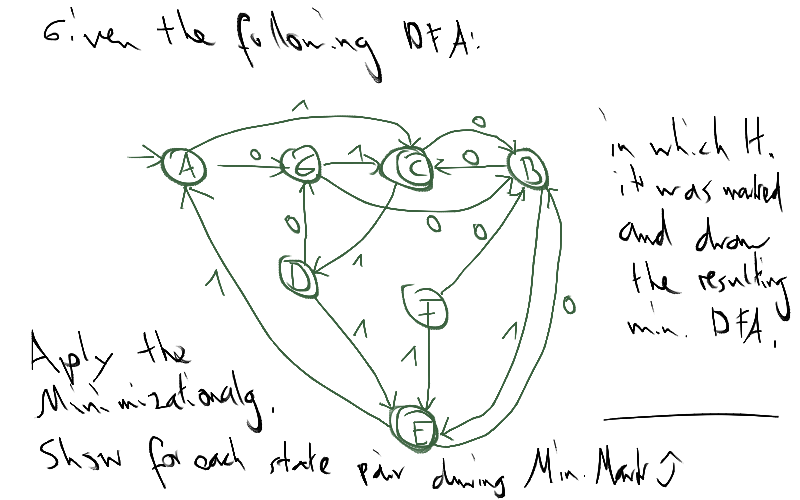
\includegraphics[width=\linewidth]{images/dfa_ex_task.png}
\caption{An example DFA minimization task.}
\label{fig:dfa_ex_task}
\end{figure}

\begin{figure}
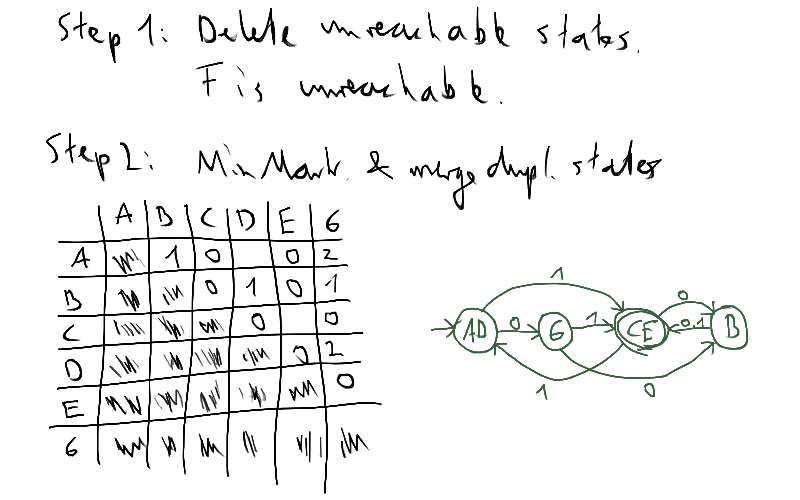
\includegraphics[width=\linewidth]{images/dfa_ex_sol.png}
\caption{Solution to the DFA minimization task in fig.~\ref{fig:dfa_ex_task}.}
\label{fig:dfa_ex_sol}
\end{figure}

\noindent Figures~\ref{fig:dfa_ex_task} and~\ref{fig:dfa_ex_sol} show such a task and solution. The students are confronted with a \emph{task DFA} $A_{task}$. Firstly, unreachable states have to be eliminated, we then gain the \emph{reachable DFA} $A_{re}$. Secondly equivalent state pairs of $A_{re}$ are merged such that the minimal \emph{solution DFA} $A_{sol}$ is found. The table $T$ displayed in figure~\ref{fig:dfa_ex_sol} is nothing else but a visualization of the function $m$, whereas $T(q_0, q_1) = i \Leftrightarrow (q_0, q_1) \in m(i)$.

We do some rather formal statements and requirements. Firstly, we can state that
\begin{itemize}
	\item $A_{re} = \RemUnr(A_{task}, \CompUnr(A_{task}))$ and
	\item $A_{sol} = \RemEq(A_{re}, \CompDist(A_{re}))$
\end{itemize}
Therefore $A_{sol}$ is minimal regarding $A_{re}$ and $A_{task}$. Secondly the languages of $A_{task}, A_{re}$ and $A_{sol}$ are be equal. We know that \CompDist\ requires $A_{re}$ to be complete and that \RemEq\ creates complete DFAs, so $A_{sol}$ is complete too. Furthermore we know that every state of $A_{re}$ is reachable since it is the output of \RemUnr.

\gregor{How to define 'already found DFA sol' as requirement. Final states argument missing.}

\subsection{Difficulty adjustment possibilities}

Concerning the execution of \MinAlg\ we find that its difficulty can be classified through various classification numbers.

\paragraph*{\CompDist-depth ($\mmD(A_{task})$).}

Consider the computation of the sets $m(i)$ in \CompDist. Determining $m(0)$ is quite straightforward, because it consists simply of tests whether two states are in $F \times Q \setminus F$ (see~\ref{ch:1:m-minmark}, line 3). Determining $m(1)$ is less easy: The rule for determining all $m(i), i > 0$ is different to that for $m(0)$ and more complicated (see~\ref{ch:1:m-minmark}, line 6). Determining $m(2)$ requires the same rule. It shows nonetheless a students understanding of the terminating behavior of \CompDist: It does not stop after computing $m(1)$, but only when no more distinguishable state pairs were found. Concerning the sets $m(i), i > 2$ however no additional understanding can be shown.

It would therefore be sensible if $\mmD(A_{task})$ could be adjusted for example by parameters $m_{min}, m_{max}$ which give lower and upper bounds for that value.

\paragraph*{Number of states ($\mathcal{Q}_{sol}, \mathcal{Q}_{eq}, \mathcal{Q}_{unr}$).}

To control the number of states in $A_{task}, A_{re}$ and $A_{sol}$, we will introduce three parameters: $\mathcal{Q}_{sol}, \mathcal{Q}_{eq}, \mathcal{Q}_{unr} \in \mathbb{N}$. These parameters get their meaning by the following equations:
\begin{align*}
    |Q_{sol}| &= \mathcal{Q}_{sol} \\
    |Q_{re}| &= \mathcal{Q}_{sol} + \mathcal{Q}_{eq} \\
    |Q_{task}| &= \mathcal{Q}_{sol} + \mathcal{Q}_{eq} + \mathcal{Q}_{unr}
\end{align*}
It is sensible to have $\mathcal{Q}_{unr} > 1, \mathcal{Q}_{eq} > 1$, such that \RemUnr\ and \RemEq\ will not be skipped. To not make the task trivial, $\mathcal{Q}_{sol} > 2$ is sensible. An exercise instructor will find it useful, to control exactly how big $\mathcal{Q}_{unr}$, $\mathcal{Q}_{eq}$ and $\mathcal{Q}_{sol}$ are: The higher $\mathcal{Q}_{unr}, \mathcal{Q}_{eq}$, the more states have to be eliminated and merged. The higher $\mathcal{Q}_{sol} + \mathcal{Q}_{eq}$, the more state pairs have to be checked during \CompDist.

\gregor{Concept for min max.}
%To control the number of states in $A_{task}, A_{re}$ and $A_{sol}$, we will introduce three pairs of parameters, denoting each ranges: $Q_{s,min}, Q_{s,max}$ for the number of states in the solution DFA, $Q_{e,min}, Q_{e,max}$ for the number of equivalent state pairs in $A_{re}$ and $A_{task}$, and $Q_{u,min}, Q_{u,max}$ for the number of unreachable states in $A_{task}$. Consequently the following equations are true:
%\begin{align*}
%|Q_{sol}| &\in [Q_{s,min}, Q_{s,max}] \\
%|Q_{re}| &= |Q_{sol}| + n \in [Q_{e,min}, Q_{e,max}] \\
%|Q_{task}| &= |Q_{re}| + n \in [ Q_{u,min}, Q_{u,max}]
%\end{align*}

\paragraph*{Alphabet size.}

The more symbols the alphabet of $A_{task}, A_{re}$ and $A_{sol}$ has (note how \MinAlg\ does not change the alphabet), the more transitions have to be followed when checking whether $(\delta(q,\sigma),\delta(p,\sigma))\in m(i-1)$ is true for each state pair $p,q$.

\paragraph*{Completeness of $A_{task}$.}

Even though \CompUnr\ and \RemUnr\ do not require their input DFA $A_{task}$ to be complete, it is sensible to build it that way. The implications of the completeness-property are - in comparison to the other concepts involved here - rather subtle. This is especially due to its purely representational nature, a DFA has the same language and $\mmD$-value, whether it is represented in its complete form or not. Nonetheless we shall introduce a parameter $c$, that determines if there exist unreachable states, that make $A_{task}$ incomplete. Thus an exercise lecturer could showcase this matter on a DFA and generate according exercises.

\paragraph*{Planar drawing of $A_{task}$.}

A graph $G$ is \emph{planar} if it can be represented by a drawing in the plane such that its edges do not cross. Such a drawing is then called \emph{planar drawing} of $G$. A visual aid for students would be given, if the task DFA were planar and presented as a planar drawing. In this work libraries and parameters $p_1, p_2 \in \{0,1\}$ (toggling planarity of $A_{sol}, A_{task}$) will be used to allow the option of planarity, but neither ensuring planarity nor planar drawing will be investigated further theoretically.

\paragraph*{Maximum degree of any state in $A_{task}$.}

The \emph{degree} $deg(q)$ of a state $q \in Q$ in a DFA $A$ is defined as $deg(q) = |d^-(q)| + |d^+(q)|$, so the total number of transitions in which $q$ participates. By capping the maximum degree for all states, the graphical representation of the DFA would be more clear. In this work the inclusion of a maximum degree parameter is omitted.

%Note that $deg(q) \geq |\Sigma|$ for any complete DFA, since states of complete DFAs have to use all alphabet symbols on outgoing transitions.

\subsection{Summary of found criteria}

\gregor{TODO}

\label{ch:1:determined-requirements}
Accepted general criteria:
\begin{itemize}
	\item[->] $L(A_{sol}) = L(A_{re}) = L(A_{task})$
	\item[->] $\mmD(A_{sol}) = \mmD(A_{re}) = \mmD(A_{task})$
\end{itemize}
Accepted solution DFA criteria:
\begin{itemize}
	\item[->] has to be minimal, complete
	\item[->] number of essential states
	\item[->] number of \CompDist\ iterations ($\mmD(A_{sol})$)
	\item[->] alphabet size
	\item[->] number of accepting states
	\item[->] planarity
	\item[->] $A_{sol}$ is new
	
	\begin{definition}[New DFAs] \label{ch:1:new-dfa}
		A DFA $A_{sol}$ is \emph{new} if it is not practically isomorph to any previously generated solution DFA.
	\end{definition}
\end{itemize}
Accepted reachable DFA criteria:
\begin{itemize}
	\item[->] has to be complete
	\item[->] number of unreachable states
	\item[->] planarity (can be checked in $O(|Q_{task}|)$)
\end{itemize}
Accepted task DFA criteria:
\begin{itemize}
	\item[->] number of states that are added to create equivalent state pairs
	\item[->] planarity
	\item[->] completeness
\end{itemize}

\section{Approach and general algorithm}

In this work we will first build the solution DFA (step 1), and - based on that - the task DFA by creating equivalent states and adding unreachable states (step 2). Both steps will fulfill all criteria chosen above and are covered in depth in chapter~\ref{ch:2} respectively chapter~\ref{ch:3}.

It follows that $\mmD$ and $L$ of both DFAs will be set when building $A_{sol}$. We know that creating equivalent states and adding unreachable does not change $L(A_{task})$ in comparison to $A_{sol}$, else \MinAlg\ would not work (a minimal DFA has in particular the same language as the original DFA). However we must ensure, that adding those states does not change $\mmD$. Since unreachable states are eliminated before \CompDist\ is applied, we need only to ensure, that creating equivalent states does not change the $\mmD$-value. We will do this during the discussion of step 2, more specifically in section~\ref{ch:3:sec-D-proof}.

At the beginning of chapter 2 and 3, we will provide formal problem definitions for both steps, that specify precisely all requirements. Here we shall content ourselves with the definition of the main algorithm:
\vspace{0.2cm}
\begin{algorithmic}[1]
	\Function{GenerateDFAMinimizationProblem}{$\mathcal{Q}_{sol}, a, f, m_{min}, m_{max}, p_1, p_2, \mathcal{Q}_{eq},\mathcal{Q}_{unr}, c$}
	\State $A_{sol} \gets \textsc{GenerateNewMinimalDFA}(\mathcal{Q}_{sol}, a, f, m_{min}, m_{max}, p_1)$
	\State $A_{task} \gets \textsc{ExtendMinimalDFA}(A_{sol}, p_2, \mathcal{Q}_{eq},\mathcal{Q}_{unr}, c)$
	\State \Return $A_{sol}, A_{task}$
	\EndFunction
\end{algorithmic}



	% !TeX spellcheck = en_US

\chapter{Generating minimal DFAs} \label{ch:2}

We seek algorithms for generation of minimal DFAs that fulfilling the conditions defined in the requirements analysis section~\ref{ch:1:requirements-analysis}. We formally subsume these conditions via the GenerateNewMinimalDFA-problem:
\begin{definition}[GenerateNewMinimalDFA] $ $ \\
	$ $ \vspace{-0.4cm} \\
	\noindent $\underline{\emph{Given:}}$
	\vspace{-0.5cm}
	\begin{align*}
	\mathcal{Q}_{sol} \in \mathbb{N}\ \ \ & \emph{number of states} \\
	a \in \mathbb{N}\ \ \ & \emph{alphabet size} \\
	f \in \mathbb{N}\ \ \ & \emph{number of final states} \\
	m_{min}, m_{max} \in \mathbb{N}\ \ \ & \emph{lower and upper bound for $\mmD$-value} \\
	p \in \{0,1\}\ \ \ & \emph{planarity-bit}
	\end{align*}
	\noindent $\underline{\emph{Task:}}$ \emph{Compute, if it exists, a solution DFA $A_{sol}$ with}
	\begin{itemize}
		\item $|Q_{sol}|=\mathcal{Q}_{sol}$, $|\Sigma_{sol}|=a$, $|F_{sol}|=f$
		\item $m_{min} \le \mmD(A_{sol}) \le m_{max}$
		\item $A_{sol}$ \emph{being planar iff} $p = 1$
		\item $A_{sol}$ \emph{being new}
	\end{itemize}
\end{definition}
\noindent We consider different approaches to solve this problem, of which those using trial-and-error will be discussed most broadly.

Note that the presented algorithms will not be able to compute all of $\mathfrak{A}_{min}$ since we are going to exclude minimal DFAs that are practical isomorph to already found ones.

\section{Using trial and error}

We will develop an algorithm that makes partly use of the trial-and-error paradigm to find matching DFAs. The approach here is as follows:

Firstly a \emph{test} DFA $A_{test}$ is generated by use of either randomness or enumeration. Alphabet size and number of (final) states will already be correct. On this DFA then tests will be executed, to check if it is minimal, planar (if wished) and new. If this is the case, $A_{test}$ will be returned, if not, new test DFAs are generated until all tests pass.

By constructing test DFAs with already correct alphabet size and number of (final) states we are able to subdivide the search space of DFAs in advance into much smaller pieces which are in particular finite.

\gregor{How much smaller? Why now finite?}

\vspace{0.2cm}
\begin{algorithmic}[1]
	\Function{BuildNewMinimalDFA-1\ }{$\mathcal{Q}_{sol}, a, f, m_{min}, m_{max} \in \mathbb{N}, p \in \{0,1\}$}
		\While {True}
		
			\vspace{0.2cm}
		
			\State generate DFA $A_{test}$ with $|Q|, |\Sigma|, |F|$ matching $\mathcal{Q}_{sol}, a, f$
			
			\vspace{0.2cm}
			
			\If {$A_{test}$ not minimal \textbf{or not} $m_{min} \leq \mmD(A_{test}) \leq m_{max}$}
				\State \textbf{continue}
			\EndIf
			
			\If {$p = 1$ \textbf{and} $A_{test}$ is not planar}
				\State \textbf{continue}
			\EndIf
			
			\If {$A_{test}$ is not new}
				\State \textbf{continue}
			\EndIf
			
			\vspace{0.2cm}
			
			\State\Return $A_{test}$
		\EndWhile
	\EndFunction
\end{algorithmic}
\vspace{0.2cm}
We will complete this algorithm by resolving how the tests in lines $4, 6$ and $8$ work and by showing two methods for generation of automatons with given restrictions of $|Q|, |\Sigma|$ and $|F|$.

\subsection{Ensuring $A_{test}$ is minimal and $\mmD(A_{test})$ is correct}

In order to test, whether $A_{test}$ is minimal, we could simply use the minimization algorithm and compare the resulting DFA and $A_{test}$ using an isomorphy test. However it is sufficient to ensure, that no equivalent or unreachable states exist.
\gregor{minimality planarity complete under isomorphy}

To get $\mmD(A_{test})$, we have to run \CompDist\ entirely anyway. Hence we can combine the test for equivalent states with computing the DFAs $\mmD$-value:
\vspace{0.2cm}
\begin{algorithmic}[1]
	\Function{HasEquivalentStates}{$A$}
		\State $depth \gets 0$
		\State $M \gets \{ (p,q), (q,p)\ |\ p \in F, q \notin F \}$
		\Do
			\State $depth \gets depth + 1$
			\State $M' \gets \{ (p,q)\ |\ (p,q) \notin M \land \exists \sigma \in \Sigma \colon (\delta(p,\sigma), \delta(q,\sigma)) \in M \}$
			\State $M \gets M \cup M'$
		\doWhile {$M' \neq \emptyset$}
		\State $hasDupl \gets | \{ (p,q)\ |\ p \neq q \land (p,q) \notin M \} | > 0$
		\State \Return $hasDupl, depth$
	\EndFunction
\end{algorithmic}
\vspace{0.2cm}
Since \CompDist\ basically computes all distinguishable state pairs $\not\sim_A$, we test in line $9$, whether there is a pair of distinguishable states not in $\not\sim_A$.

Regarding the unreachable states, we can just use \CompUnr\ and test whether the computed set is empty:
\vspace{0.2cm}
\begin{algorithmic}[1]
	\Function{HasUnreachableStates}{$A$}
	\State \Return $|\CompUnr(A)| > 0$
	\EndFunction
\end{algorithmic}

\subsection{Ensuring $A_{test}$ is planar}

There exist several algorithms for planarity testing of graphs. In this work, the library \emph{pygraph}\footnote{\url{https://github.com/jciskey/pygraph}} has been used, which implements the Hopcroft-Tarjan planarity algorithm. More information on this can be found for example in this~\cite{Koc93} introduction from William Kocay. The original paper describing the algorithm is~\cite{HT74}.

\subsection{Ensuring $A_{test}$ is new}

In our requirements we stated, that we wanted the generated solution DFA to be new, meaning not practically isomorph to any previously generated solution DFA. This implies the need of a database, that allows saving and loading DFAs. We name this database \emph{DB1}. Assuming the database is relational, the following scheme is proposed:
\begin{center}
	\begin{tabular}{c c c c c c}
	$|Q_A|$ & |$\Sigma_A$| & $|F_A|$ & $\mmD(A)$ & $isPlanar(A)$ & $encode(A)$
	\end{tabular}
\end{center}
With this scheme we can fetch once all DFAs matching the search parameters. Thus we need not fetch all previously found DFAs every time, but only those that are relevant. Afterwards we must only check whether any practical isomorphy test on the current test DFA and one of the fetched DFAs is positive. If any test DFA passes all tests and is going to be returned, then we have to save that DFA in the database.

A more concrete specification of this proceeding is shown below, embedded in the main algorithm:
\vspace{0.2cm}
\begin{algorithmic}[1]
	\Function{BuildNewMinimalDFA-2\ }{$\mathcal{Q}_{sol}, a, f, m_{min}, m_{max}, p$}
	
		\vspace{0.2cm}
	
		\State $l \gets$ all DFAs in DB1 matching $\mathcal{Q}_{sol}, a, f, m_{min}, m_{max}, p$
		
		\vspace{0.2cm}
		
		\While {True}
		
		\vspace{0.2cm}
		
			\State $\ldots$
			\If {$A_{test}$ is practical isomorph to any DFA in $l$}
				\State \textbf{continue}
			\EndIf
			
			\vspace{0.2cm}
			
			\State save $A_{test}$ and its respective properties in DB1
			\State\Return $A_{test}$
		\EndWhile
	\EndFunction
\end{algorithmic}
\vspace{0.2cm}

\subsection{Option 1: Generating $A_{test}$ via Randomness}

We now approach the task of generating a random DFA whereas alphabet and number of (final) states are set.

Corollary~\ref{ch:1:cor:all-min-dfa-ism} tells us, that the states names are irrelevant for the minimality of a DFA, therefore we will give our generated DFAs simply the states $e_1, \ldots, e_{\mathcal{Q}_{sol}}$. For alphabet symbols this is not given. But since we \gregor{TODO minimality and planarity complete under isomorphy}

We can state, that our start state is $e_1 \in Q$, since we can apply an isomorphism to every DFA, such that its start state is renamed to $e_1$.

The remaining elements that need to be defined are $\delta$ and $F$. The set of final states is supposed to have a size of $f$ and be a subset of $Q$. Therefore we can simply choose randomly $f$ distinct states from $Q$.

The transition function has to make the DFA complete, so we have to choose an ``end'' state for every combination in $Q \times \Sigma$. There is no restriction as to what this end state shall be, so given $e \in Q$ and $\sigma \in \Sigma$ we can randomly choose an end state from $Q$.

With defining how to compute $\delta$ we have covered all elements of a DFA.

\vspace{0.2cm}
\begin{algorithmic}[1]
	\Function{BuildNewMinimalDFA-3a\ }{$\mathcal{Q}_{sol}, a, f, m_{min}, m_{max}, p$}
	
		\vspace{0.2cm}
	
		\State $l \gets$ all DFAs in DB1 matching $\mathcal{Q}_{sol}, a, f, m_{min}, m_{max}, p$
		\State $Q \gets \{e_1, \ldots, e_{\mathcal{Q}_{sol}}\}$
		\State $\Sigma \gets \{\sigma_1, \ldots, \sigma_a\}$
		
		\vspace{0.2cm}
		
		\While {True}
		
		\vspace{0.2cm}
		
			\State $\delta \gets \emptyset$
			\For {$e$ \textbf{in} $Q$}
				\For {$\sigma$ \textbf{in} $\Sigma$}
					\State $e' \gets$ random chosen state from $Q$
					\State $\delta \gets \delta \cup \{((e,\sigma),e')\}$
				\EndFor
			\EndFor
			\State $s \gets e_1$
			\State $F \gets$ random sample of $f$ states from $Q$
			\State $A_{test} \gets (Q, \Sigma, \delta, s, F)$
			
			\vspace{0.2cm}
			
			\If {$A_{test}$ not minimal \textbf{or not} $m_{min} \leq \mmD(A_{test}) \leq m_{max}$}
			\State \textbf{continue}
			\EndIf
			
			\If {$p = 1$ \textbf{and} $A_{test}$ is not planar}
			\State \textbf{continue}
			\EndIf
			
			\If {$A_{test}$ is isomorph to any DFA in $l$}
			\State \textbf{continue}
			\EndIf
			
			\vspace{0.2cm}
			
			\State save $A_{test}$ and its respective properties in DB1
			\State\Return $A_{test}$
		\EndWhile
	\EndFunction
\end{algorithmic}
\vspace{0.2cm}

\subsection{Option 2: Generating $A_{test}$ via Enumeration}

% enumerating instead of random

The second method of test DFA generation is based on the idea, that instead of randomly generating $F$ and $\delta$, we could just enumerate through all possible final state sets and transition functions.

% finite enumerations, how many

Both enumerations are finite, given $\mathcal{Q}_{sol}$ and $a$. Having a requirement of $f$ final states, then $\mathcal{Q}_{sol}$ choose $f$ is the number of possible $F$-configurations. On the other hand there are ${\mathcal{Q}_{sol}}^{\mathcal{Q}_{sol}*a}$ possible $\delta$-configurations: We have to choose one of $\mathcal{Q}_{sol}$ possible end states for every combination in $Q\times\Sigma$ - so $\mathcal{Q}_{sol}*a$ times.

% Two fields

Again we will call our states and symbols w.l.o.g.\ $e_1,\ldots,e_{\mathcal{Q}_{sol}}$ resp.\ $\sigma_1,\ldots,\sigma_a$. We will represent the state of an enumeration with two fields $F_F$ and $F_\delta$. The first field shall have $\mathcal{Q}_{sol}$ Bits, whereas Bit $F_F[i] \in [0,1]$ represents the information, whether $e_i$ is a final state or not. The second field shall have $\mathcal{Q}_{sol}*a$ entries containing state indices, such that entry $F_\delta[i * a + j] = k, k\in[1,\mathcal{Q}_{sol}]$ says, that $\delta(e_i, \sigma_j) = e_k$. These semantics are illustrated in figure~\ref{fig:dfa_enum_bit_fields}.

% -- EX example of the two fields and their meaning

\begin{figure}
	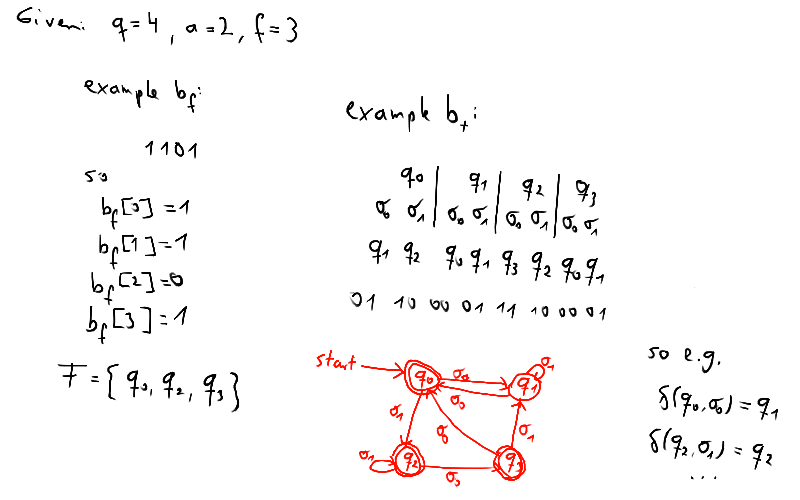
\includegraphics[width=\linewidth]{images/dfa_enum_bit_fields.png}
	\caption{Example for two possible configurations of the fields $F_F$ and $F_\delta$ given $\mathcal{Q}_{sol}, a$ and $f$. Below the corresponding DFA is drawn.}
	\label{fig:dfa_enum_bit_fields}
\end{figure}

% how to compute next DFA

Given an enumeration state $b_f, b_t$ and $\mathcal{Q}_{sol}, a, f$ we will then compute the next DFA based on this state as follows. We will treat both fields as numbers, $F_f$ as binary and $F_\delta$ as $\mathcal{Q}_{sol}$-ary. To get to the next DFA, we will first increment $F_\delta$ by $1$. If $F_\delta = 1 \ldots 1$, then we increment $F_F$ until it contains $f$ ones (again) and set $F_\delta$ to $0 \ldots 0$. This behavior is summarized in the following algorithm: \gregor{Clarify what happens at 11111...}
\vspace{0.2cm}
\begin{algorithmic}[1]
	\Function{IncrementEnumProgress\ }{$F_F, F_\delta, \mathcal{Q}_{sol}, a, f$}
	\State add $1$ to $(F_\delta)_{\mathcal{Q}_{sol}}$
	\If {$F_\delta = 0 \ldots 0$}
		\While {$\#_1(F_F) \neq f$} \Comment{if the number of 1s in $F_F$ is not $f$}
			\State add $1$ to $(F_F)_2$
			\If {$F_F = 0\ldots 0$}
				\State \Return $\bot$
			\EndIf
		\State $F_\delta = 0 \ldots 0$
		\EndWhile
	\EndIf
	\State \Return $F_F, F_\delta$
	\EndFunction
\end{algorithmic}
\vspace{0.2cm}
The example in figure~\ref{fig:dfa_enum_incr} illustrates such increments.

% EX -- example of an enumProgress increment

\begin{figure}
	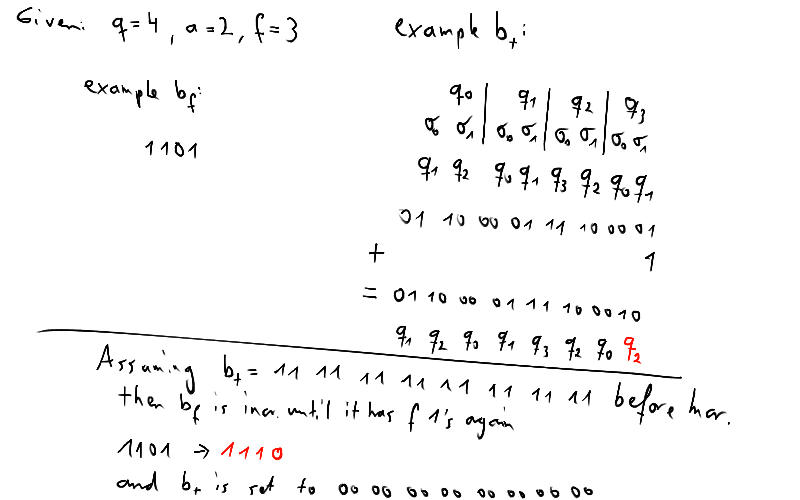
\includegraphics[width=\linewidth]{images/dfa_enum_incr.png}
	\caption{The upper half shows how a $F_\delta$-increment results in a change in the resulting DFAs transition function: $\delta(e_3, \sigma_1) = e_1$ becomes $\delta(e_3, \sigma_1) = e_2$. The lower half shows what happens, if $F_\delta$ has reached its end.}
	\label{fig:dfa_enum_incr}
\end{figure}

Based on the incremented bit-fields the new DFA can be build according to the semantics defined above:
\vspace{0.2cm}
\begin{algorithmic}[1]
	\Function{DFAfromEnumProgress\ }{$F_F, F_\delta, \mathcal{Q}_{sol}, a, f$}
	\State $Q \gets \{e_1, \ldots, e_{\mathcal{Q}_{sol}}\}$
	\State $\Sigma \gets \{\sigma_1, \ldots, \sigma_a\}$
	\State $\delta \gets \emptyset$
	\For {$i$ \textbf{in} $[1, \ldots, \mathcal{Q}_{sol}]$}
		\For {$j$ \textbf{in} $[1, \ldots, a]$}
            \State $\delta(e_i, \sigma_j) = e_{F_\delta[i * a + j]}$
		\EndFor
	\EndFor
	\State $s \gets e_1$
	\State $F \gets \{\ e_i\ |\ i \in [1, \ldots, \mathcal{Q}_{sol}] \land F_F[i] = 1\ \}$
	\State \Return $(Q, \Sigma, \delta, s, F)$
	\EndFunction
\end{algorithmic}
\vspace{0.2cm}
The initial field values are each time $0\ldots 0$. Note how construction and use of these fields results in DFAs with correct alphabet size and number of (final) states. An enumeration can finish either because a matching DFA has been found or all DFAs have been enumerated.

% saving enumProgress for later progression

Once the enumeration within a call of \textsc{BuildNewMinimalDFA} has been finished, it is reasonable to \emph{save} the enumeration progress (meaning the current content of $F_F, F_\delta$), such that during the next call enumeration can be resumed from that point on. The alternative would mean, that the enumeration is run in its entirety until that point again, whereas all so far found DFAs would be found to be not new. Thus we introduce a second database $DB2$ with the following table:
\begin{center}
	\begin{tabular}{c c c c c c}
		$|Q_A|$ & |$\Sigma_A$| & $F_F$ & $F_\delta$
	\end{tabular}
\end{center}
We reduce the enumeration room for each calculation.
\vspace{0.2cm}
\begin{algorithmic}[1]
	\Function{BuildNewMinimalDFA-3b\ }{$\mathcal{Q}_{sol}, a, f, m_{min}, m_{max}, p$}
	
		\vspace{0.2cm}
	
		\State $l \gets$ all DFAs in DB1 matching $\mathcal{Q}_{sol}, a, f, m_{min}, m_{max}, p$
		\State $F_F, F_\delta \gets$ load enumeration progress for $\mathcal{Q}_{sol}, a, f, p$ from DB2
		
		\vspace{0.2cm}
		
		\While {True}
		
			\vspace{0.2cm}
		
			\If {$F_F, F_\delta$ is finished}
				\State save $F_F, F_\delta$
				\State\Return $\bot$
			\EndIf
			\State $A_{test} \gets$ next DFA based on $F_F, F_\delta$
			
			\vspace{0.2cm}
			
			\If {$A_{test}$ not minimal \textbf{or not} $m_{min} \leq \mmD(A_{test}) \leq m_{max}$}
				\State \textbf{continue}
			\EndIf
			
			\If {$p = 1$ \textbf{and} $A_{test}$ is not planar}
				\State \textbf{continue}
			\EndIf
			
			\If {$A_{test}$ is isomorph to any DFA in $l$}
				\State \textbf{continue}
			\EndIf
			
			\vspace{0.2cm}
			
			\State save $F_F, F_\delta$ in DB2
			\State save $A_{test}$ and its respective properties in DB1
			\State\Return $A_{test}$
		\EndWhile
	\EndFunction
\end{algorithmic}
\vspace{0.2cm}

\section{Alternative approach: Building $m(i)$ bottom up}

Build $m$ from $m$-\CompDist\ iteratively. (Why would this basically result in running \CompDist\ all the time?)

\section{Related research on DFA generation}

Nicaud provides an overview of results on random generation and combinatorial properties of DFAs in ~\cite{Nic14}. We will outline relevant related research.

%\subsection{}

Nicaud's summary indicates, that research has focused on randomized generation of accessible, but not minimal DFAs so far. In the following we will sketch some approaches that have come up.

\paragraph*{Using the recursive method.}

Champarnaud and Paranthoën~\cite{CP05} continue ideas started by Nicaud in his thesis~\cite{Nic00}. Let $\mathfrak{F_{n,m}}$ be the set of extended $m$-ary trees of order $n$. These trees are characterized by a partitioning $V = N \uplus L$ with $|N| = n$ and $v \in N \Rightarrow d^+(v) = m$ and $v \in L \Rightarrow d^+(v) = 0$. We define the following set of tuples using $s=n(m-1)$:
\[
    \mathfrak{R_{m,n}} = \{\ (k_1,\ldots,k_s) \in \mathbb{N}^s\ |\ \forall i\in [2,s]\colon k_i \geq \left\lceil\frac{i}{m-1}\right\rceil\ and\ k_i \geq k_{i-1}\ \}
\]
In~\cite[p. 6]{CP05} it is shown that there exists a bijection $\varphi$ between $\mathfrak{F_{n,m}}$ and $\mathfrak{R_{m,n}}$ which maps to $k_i$, $i\in[1,s]$ of a tuple the number of leaves visited before the $i$th leaf in a tree. The connection to accessible DFAs is established by proving that  ``transition structures\footnotemark''\ with $|Q|=n$, $|\Sigma|=m$ reduced to the set of the smallest paths from the $s$ to each other state are in bijection with extended $m$-ary trees of order $n$ (see~\cite[p. 8]{CP05}).

As a consequence they are able to construct a random generation of accessible complete DFAs using the ``recursive method'' from~\cite{NW78} which generates $n$-tuples~\cite[p. 10]{CP05}. Nicaud states in his survey that the algorithm's runtime is $\mathcal{O}(n^2)$ but notes, that generation of DFAs with more than ``a few thousand states'' is practically hard to do~\cite[pp. 10-11]{Nic14}.
\footnotetext{Those are essentially DFAs without final state sets.}

Almeida et.\ al.~\cite{AAA09, AMR09, RMA05} present and implement methods using a string-encoding of DFAs for exact enumeration and random generation of DFAs. Nicaud~\cite[p. 11]{Nic14} states in a remark, that this approach uses the same recursive method and differs only in the DFA encoding.

\paragraph*{Using Boltzmann sampler.}

Bassino, David and Nicaud present and implement a more efficient random generator of accessible complete DFAs in~\cite{BDN07, BN07}. Their idea is based on so called Boltzmann samplers. This framework of samplers is characterized in particular by the fact that the size of its generated objects are not fixed but in an interval around a given input size - this stands in opposition to most random generators in literature~\cite[p. 2]{DFL04}.

In~\cite{BN07} the authors use a Boltzmann sampler to generate set partitions that are shown to be in bijection with so called box diagrams~\cite[p. 8]{BN07} which are in turn in bijection to accessible complete DFAs~\cite[p. 4]{BN07}. They thus acquire an average runtime complexity of $\mathcal{O}(n^{3/2})$ for a single random generation.

\paragraph*{Using a rejection algorithm.}

Carayol and Nicaud~\cite{CN12} give a simple algorithm with the same runtime complexity. They use a result stating that the size of accessible DFAs is concentrated around some computable value. In the end random possibly inaccessible DFAs of a specific size are generated, of which afterwards all unreachable states are deleted. This is thus essentially a rejection algorithm with clever generation of test DFAs. They furthermore show that allowing approximate sampling with the number of states being in $[n-\varepsilon\sqrt{n}, n+\varepsilon\sqrt{n}]$ results in linear expected runtime.

\paragraph*{Others and comparison to algorithm presented in this work.}

In his survey Nicaud mentions a paper by Bassino and Sportiello~\cite{BS13} that yields random generation of accessible DFAs in expected linear time. This work will not be discussed further here.

In this work we use a rejection algorithm that generates test DFAs either by randomization or by enumeration. Both methods implement a naive approach. The generated test DFAs are not necessary minimal and in particular not necessary accessible as in~\cite{CN12}. The enumeration method uses encodings of DFAs similar to those used by Almeida et.\ al.~\cite{RMA05}.


\section{Empirical and combinatorial results}

Concerning combinatorial properties of DFAs, several authors (e.g.~\cite{BN07, DKS02, HJ14}) consider a work from Vyssotsky~\cite{Vys59} in the Bell laboratories to be the first on this subject. A contribution by Korshunov~\cite{Kor78} is often cited in this regard, for he firstly ``determines an asymptotic estimate of the number of accessible complete and deterministic $n$-state automata over a finite alphabet''~\cite{BDS11}.

Implementations (e.g.~\cite{AAA09, BDN07}) of various random and enumeration generation methods have given rise to several empirical observations concerning the number of minimal DFAs, their fraction among all DFAs and so forth.

Domaratzki, Kisman, and Shallit~\cite{DKS02} give some asymptotic estimates and explicit computations for the number of each several types of languages and automata that are distinct. The here relevant results have been subsumed and extended in~\cite[p. 8]{AMR09} by means of exact enumeration and are confirmed in~\cite{BDN07}.

\begin{figure}[H]
	\centering
	\begin{tabular}{|c|c|l|l|l|}
		\hline
		$|\Sigma|$ ($k$) & $|Q|$ ($n$) & $|\mathcal{A}_{min,n,k}|$ & $|\mathcal{A}_{n,k}|$ & Minimal \% \\\hline
		
		$k = 2$ & $2$ & \textbf{24} & 64 & 0.38 \\
		& $3$ & \textbf{1028} & 5832 & 0.18 \\
		& $4$ & \textbf{56014} & 1048576 & 0.05 \\
		& $5$ & \textbf{3705306} & 312500000 & 0.01 \\
		& $6$ & \textbf{286717796} & 139314069504 & 0.0 \\
		& $7$ & \textbf{25493886852} & 86812553324672 & 0.0 \\\hline
		
		$k = 3$ & $2$ & \textbf{112} & 256 & 0.44 \\
		& $3$ & \textbf{41928} & 157464 & 0.27 \\
		& $4$ & \textbf{26617614} & 268435456 & 0.1 \\
		& $5$ & \textbf{25184560134} & 976562500000 & 0.03 \\\hline
		
		$k = 4$ & $2$ & \textbf{480} & 1024 & 0.47 \\
		& $3$ & \textbf{1352732} & 4251528 & 0.32 \\
		& $4$ & \textbf{7756763336} & 68719476736 & 0.11 \\\hline
		
		$k = 5$ & $2$ & \textbf{1984} & 4096 & 0.48 \\
		& $3$ & \textbf{36818904} & 114791256 & 0.32\\\hline
	\end{tabular}
	\caption{Table depicting the amount of minimal complete DFAs among all complete DFAs for various sizes of $Q, \Sigma$. The numbers of minimal DFAs (bold numbers) are taken from~\cite[p. 8]{AMR09}.}
	\label{fig:dfa_minimal_ratios}
\end{figure}

\noindent In table~\ref{fig:dfa_minimal_ratios} we use these results to determine the ratios of minimal complete DFAs among all complete DFAs for given $|Q|$ and $|\Sigma|$. The number of all DFAs is computed as follows:
\[
|\mathcal{A}_{n,k}| = \underbrace{n^{n*k}}_{\#\text{possible }\delta\text{'s}} * \underbrace{2^n}_{\#\text{possible sets }F}
\]
Thus we gain an insight into how probable the generation of a distinct minimal test DFA is without applying further constraints. For our proposed default parameters $n\in[4-5]$ and $k\in[2-3]$ the probabilities of successful generation range from $1\%$ to $5\%$. Practical tests have shown that this leads to sufficient short run times for our implementation.

Further interesting results in this area include the determination of the fraction of minimal automata among accessible complete DFAs~\cite{BDS11} and asymptotic estimates for the number of states that a random minimized DFA has~\cite{BK13}.

	% !TeX spellcheck = en_US

\chapter{Extending solution DFAs to task DFAs} \label{ch:3}

Given a solution DFA $A_{sol}$ we have determined the following requirements for generating a task DFA $A_{task}$ in our requirements analysis (see~\ref{ch:1:determined-requirements}):
\begin{itemize}
	\item[->] $L(A_{sol}) = L(A_{task})$
	\item[->] $\mmD(A_{sol}) = \mmD(A_{task})$
	\item[->] number of duplicate states
	\item[->] number of unreachable states
	\item[->] alphabet size
	\item[->] planarity (can be checked in $O(|Q_{task}|)$)
	\item[->] completeness (for \MinMark-algorithm to work)
\end{itemize}
In order to fulfill these requirements when adding new elements to the given minimal automaton $A_{sol}$, we simply look at how duplicate and unreachable states are removed by the minimization algorithm, such that we can deduce from their properties, which restrictions are given for adding such elements. We will show for both classes of addable elements, that they do not change the DFAs language and its $\mmD$-value.

\gregor{Adding unreachable states is essentially just talking about that special equivalence class. Think and tell more about this}

\section{Adding duplicate states}

Firstly, let us state that since unreachable states are removed first in the minimization algorithm, we may assume that every state, that is duplicated, is reachable.

\gregor{hidden definition: correct duplication}
%\begin{definition}[Correct duplication]
%	Let $A = (Q, \Sigma, \delta, s, F)$ be the solution DFA and $A' = (Q', \Sigma, \delta', s, F')$ the task DFA with a $q_o, q_d \in Q'$, $q_d \notin Q$. Building such an $A'$ is called a \emph{correct duplication}, iff
%	\[
%		d_{A'}(q_o, q_d)
%	\]
%	and
%	\[
%		\forall q \in Q \colon [q]_{d_{A'}} = [q]_{d_A}
%	\]
%\end{definition}

Step 3 and 4 of the minimization algorithm are concerned with detection and elimination of duplicate states. How do we add duplicate states to a DFA?

Consider the properties a duplicate state, say $q_d$, must have. It is in particular duplicate to \emph{another} state, we call it $q_o$. We call the new, by $q_d$ extended DFA, $A$.

%  Since we add only one state for now, $q_d$, we can assume that $q_o$ is part of the solution DFA. 

\paragraph*{Outgoing transitions}

We know that $q_d$, $q_o$ are duplicates, iff $\forall \sigma \in \Sigma \colon [\delta(q_d, \sigma)]_{d_A} = [\delta(q_o, \sigma)]_{d_A}$. Thus, when adding some $q_d$, we have to choose for each symbol $\sigma \in \Sigma$ at least one transition from the following set:
\[
	P_\sigma = \{\ ((q_d, \sigma), p)\ |\ p \in [\delta(q_o, \sigma)]_{d_A}\ \}
\]
Since the solution DFA is complete, we know that every $P_\sigma \neq \emptyset$.

\gregor{Why does this not affect the eq. class of any other state?}

\paragraph*{Ingoing transitions}

The ingoing transitions of $q_d$ are not directly restricted through the duplicateness of $q_d$ and $q_o$.

First of all, we know, that $q_o$ is reachable. We then need to give $q_d$ at least one ingoing transition. Doing this, we have to ensure, that any state $s$, that gets such an outgoing transition to $q_d$ remains in its solution equivalence class.
	
Thus a fitting state $s$ has to have a transition to some state in $[q_d]_{d_A} = [q_o]_{d_A}$ already. So, given a state $s$ with $((s, \sigma), t)$ and $t \in [q_o]_{d_A}$, we can add $((s, \sigma), q_d)$.

But this would make our new DFA a NFA. As a consequence we have to remove the original transition $((s, \sigma), t)$ each time we add an ingoing transition for a newly created duplicate state.

So we have to choose at least one transition of
\[
	\{\ ((s, \sigma), q_d)\ |\ \delta(s,\sigma) \in [q_o]_{d_A}\ \}
\]
If a $((s, \sigma), q_d)$ is chosen, remove $((s, \sigma), t)$. This leads us to the requirement, that the equivalence class of any $q_o$ has to contain at least one state with at least $2$ ingoing transitions (see fig.~\ref{fig:dfa_add_duplicate_states}). We establish the following notion to pin down this restriction:
\[
	duplicatable(q_o) = 1 \Leftrightarrow_{def} (\exists q \in [q_o]_{d_A}\colon |d^-(q)| \geq 2)
\]
\begin{figure}
	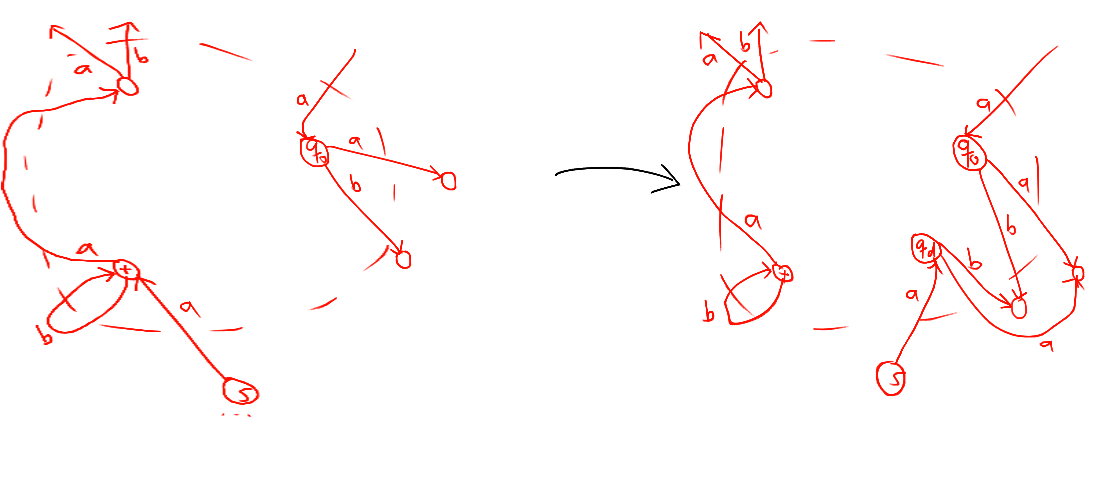
\includegraphics[width=\linewidth]{images/dfa_add_duplicate_states.png}
	\caption{If an equivalence class (here denoted by the states in the dashed area) contains a state with 2 or more ingoing transitions (in this case $t$), then a state duplicate to any of classes states may be added. Here $q_d$ is duplicate to $q_o$ and is ``stealing'' the ingoing transition $\delta(s, a)$ from $t$.}
	\label{fig:dfa_add_duplicate_states}
\end{figure}
\gregor{Talk somewhere about eq. automaton and extending it. An eq. class of reach. q's can be max. |$\Sigma$| big. From this can compute the max. number of dupl. states which can be added.}

\vspace{0.2cm}
\begin{algorithmic}[1]
	\Function{AddDuplicateStates\ }{$A_{sol}, d$}
	\State $eq\_classes \gets \{\ \{q\}\ |\ q \in Q\ \}$
	\State $eq\_class(q) = C$ such that $C \in eq\_classes$ and $q \in C$
	\State $\#_{d^-}(q) = |d^-(q)|$
	\State
	\For {$d$ \textbf{times}}
	
		\State
		\State $q_o \gets \bot$
		\For {$q$ \textbf{in} $C$}
			\If {$\#_{d^-}(q) \geq 2$}
				\State $q_0 \gets$ random chosen state from $eq\_class(q)$
				\State \textbf{break}
			\EndIf
		\EndFor
		\If {$q_o = \bot$}
			\State \Return $\bot$
		\EndIf
		
		\State
		\State $q_d \gets \max Q + 1$
		\State $Q \gets Q \cup \{ q_d \}$
		
		\State
		\For {$\sigma$ \textbf{in} $\Sigma$}
			\State $\delta(q_d, \sigma) =$ random chosen state from $eq\_class(\delta(q_o, \sigma))$
		\EndFor
		
		\State
		\State $O \gets \{\ ((s, \sigma), t) \in \delta\ |\ t \in eq\_class(q_o) \land \#_{d^-}(t) \geq 2\ \}$
		
		\State $C \gets$ random sample of at least one transition from $O$
		\For {$((s, \sigma), t)$ \textbf{in} $C$}
			\State $\delta \gets \delta \setminus \{((s, \sigma), t)\}$
			\State $\delta \gets \delta \cup \{((s, \sigma), q_d)\}$
			\State $\#_{d^-}(t) \gets \#_{d^-}(t) - 1$
			\State $\#_{d^-}(q_d) \gets \#_{d^-}(q_d) + 1$
		\EndFor
	\EndFor
	
	\State \Return $A$
	\EndFunction
\end{algorithmic}
\vspace{0.2cm}

\subsection{Adding duplicate states does not change L}

p. 159 Hopcroft

\subsection{Adding duplicate states does not change $\mmD$}

To prove this statement, we will prove two minor propositions first.

\begin{lemma}[Semantics of $(p,q) \in m(n)$] \label{ch:3:semantics-of-m(n)}
	\begin{multline*}
	(p,q) \in m(n) \Longleftrightarrow 
	\exists w\in\Sigma^*\colon |w| = n\ \land \\
	(\delta^*(p,w) \in F \Leftrightarrow \delta^*(q,w) \notin F)
	\end{multline*}
\end{lemma}

\begin{proof}
	See TI-Lecture ch. 4 ``Minimization'' p. 18.
\end{proof}

\begin{lemma}[Semantics of $\mmD(A) = n$] \label{ch:3:semantics-of-D(A)}
	\begin{multline*}
		\mmD(A) =\ n \Rightarrow \\
		n = \max_{n \in \mathbb{N}}\ \ \exists p, q \in Q\ \ \exists w \in \Sigma^* \colon |w| = n - 1\ \land \\
		(\delta^*(p,w) \in F \Leftrightarrow \delta^*(q,w) \notin F)
	\end{multline*}
\end{lemma}

\begin{proof}
	\begin{description}
		\item
		
		Via direct proof.
		
		Assume $m$-\MinMark(A) has done $n$ iterations (so $\mmD(A) = n$). We then know, that
		\begin{itemize}
			\item $\forall i \in [0,n-1]\colon m(i) \neq \emptyset$
			\item $m(n)= \emptyset$
		\end{itemize}
		$m$-\MinMark(A) terminates iff $m(i) = \emptyset$. If the first point would not hold, then the algorithm would have stopped before.
		
		Since the algorithm did $n$ iterations, the internal variable $i$ must be $n$ at the end of the last iteration. The terminating condition is $m(i) \neq \emptyset$; thus follows the second point.
		
		Recall the statement from lemma~\ref{ch:3:semantics-of-m(n)}:
		\begin{multline*}
		(p,q) \in m(n) \Longleftrightarrow 
		\exists w\in\Sigma^*\colon |w| = n\ \land \\
		(\delta^*(p,w) \in F \Leftrightarrow \delta^*(q,w) \notin F)
		\end{multline*}
	
		% a possible word per definition of D(A), m(i) and lemma
		
		Following this lemma and having $m(n-1) \neq \emptyset$ in mind, we can deduce that there exists at least one word $w\in\Sigma^*$ with $|w| = n-1$ such that for two $p,q \in Q\colon (\delta^*(p,w) \in F \land \delta^*(q,w) \notin F)$.
		
		% There is no word longer than that
		
		There cannot be any two states $p',q'\in Q$ and a word $w'\in\Sigma^*$ with $|w'| > n-1$ fulfilling this property. We could write $w'$ as $u'v'$ with $|v'| = n$. Then $m(n)$ would be non-empty, which is contradictory.
	\end{description}
\end{proof}

\begin{theorem}[]
	Adding duplicate states to an automaton $A$ does not increase the number of iterations in the \MinMark-algorithm for $A$.
\end{theorem}

\begin{proof}
	\begin{description}
		\item
		
		Proof per contradiction.
		
		Let's assume adding duplicate states $q_d^1, \ldots, q_d^n$ to a given automaton $A = (Q, \Sigma, \delta, s, F)$ results in an automaton $A' = (Q', \Sigma, \delta', s, F')$ whereas $\mmD(A) < \mmD(A')$.
		
		Concerning $A'$ we can say the following:
		\begin{itemize}
			\item $Q' = Q \cup \{ q_d^1, \ldots, q_d^n \}$
			%			\item $\delta \subseteq \delta'$
			%			\item $F \subseteq F'$
			\item W.l.o.g. $\exists q_o^1 \in Q \colon \exists q_o^2 \ldots q_o^n \in Q \colon\ d_A'(q_o^1, q_d^1), \ldots, d_A'(q_o^n, q_d^n)$
		\end{itemize}
		Let us furthermore say that $\mmD(A) = i$ and $\mmD(A') = j$. Recall now lemma~\ref{ch:3:semantics-of-D(A)}:
		\begin{multline*}
		\mmD(A) =\ n \Rightarrow \\
		n = \max_{n \in \mathbb{N}}\ \ \exists p, q \in Q\ \ \exists w \in \Sigma^* \colon |w| = n - 1\ \land \\
		(\delta^*(p,w) \in F \Leftrightarrow \delta^*(q,w) \notin F)
		\end{multline*}
		According to this lemma there must be a pair $s, t \in Q'$ to which exists a word $w \in \Sigma'^*$, $|w| = j - 1$, such that $\delta'^*(s,w) \in F' \Leftrightarrow \delta'^*(t,w) \notin F'$.
		
		Let us split $w$ as $w = uv$ such that $|v| = i$, which is exactly one symbol longer than the longest minimization word of $A$. We can formulate the following statement:
		\begin{equation}
		\text{There must exist }p, q \in Q'\text{ such that }\delta'^*(p,v) \in F' \Leftrightarrow \delta'^*(q,v) \notin F'.
		\end{equation}
		\gregor{hidden formulations here}
		%There must exist $p, q \in Q'$ such that $\delta'^*(p,v) \in F' \Leftrightarrow \delta'^*(q,v) \notin F'$.
		
		%So there exists a minimization word $v$ in $A'$, which is exactly one symbol longer than the longest minimization word of $A$. This word has length $i$ and is detected at minimization depth $i + 1$.
		
		We can therefore state, that $\neg(p \in Q \land q \in Q)$, because else $\mmD(A)$ would be higher than $i$ too.  So at least one of $p,q$ must be in $Q' \setminus Q$ which is exactly $\{ q_d^1, \ldots, q_d^n \}$.
		
		\begin{itemize}
			\item Every $q_d^k$ is $d_{A'}$-equivalent to a $q \in Q$
			\item In every case, $p,q$ can be $d_{A'}$-exchanged s.t. $p,q \in Q$
			\item But that's contradictory to $\mmD(A) = n$, because $p,q$ belong to a minimization word $w = n-1$
		\end{itemize}
		
%		Since $q_d$ is the only new state in $A'$ compared to $A$, we can conclude that at least one of both states must be $q_d$. Since $p = q_d = q$ is contradictory (\gregor{why?}), we can conclude that exactly one of both states $p, q$ is $q_d$ and that the other one is not.
%		
%		W.l.o.g.\ we say $q = q_d$ and $p \in Q' \setminus \{q_d\} = Q$ and reformulate our statement above:
%		\begin{equation}
%		\text{There must exist a }p \in Q\text{ such that }\delta'^*(p,v) \in F' \Leftrightarrow \delta'^*(q_d,v) \notin F'.
%		\end{equation}
%		\gregor{hidden formulations here}
%		
%		%Therefore we know there exists a state $p \in Q$ such that $\exists v \in \Sigma^*$, $|v| = i$ and $\delta'^*(p,v) \in F' \Leftrightarrow \delta'^*(q_d,v) \notin F'$
%		
%		Since for $q_o \in Q$ the relation $d_{A'}(q_o, q_d)$ is given, we know per definition of $d_{A'}$ that $\forall z\in\Sigma'^*\colon \delta'^*(q_o,z) \in F \Leftrightarrow \delta'^*(q_d,z) \in F$.
%		
%		This implies in combination with statement 2.2, that for $p,q_o$ the word $v\in\Sigma'^*$ would fulfill $\delta'^*(p,v) \in F' \Leftrightarrow \delta'^*(q_o,v) \notin F'$ too. But this is contradictory to $p,q \notin Q$.
	\end{description}
\end{proof}

\gregor{Old proof for one $q_d$}
%\begin{proof}
%	\begin{description}
%		\item
%		
%		Proof per contradiction.
%		
%		Let's assume adding a duplicate state $q_d$ to a given automaton $A = (Q, \Sigma, \delta, s, F)$ results in an automaton $A' = (Q', \Sigma, \delta', s, F')$ whereas $\mmD(A) < \mmD(A')$.
%		
%		Concerning $A'$ we can say the following:
%		\begin{itemize}
%			\item $Q' = Q \cup \{ q_d \}$
%			%			\item $\delta \subseteq \delta'$
%			%			\item $F \subseteq F'$
%			\item $\exists q_o \in Q \colon\ d_A'(q_o, q_d)$
%		\end{itemize}
%		Let us furthermore say that $\mmD(A) = i$ and $\mmD(A') = j$. Recall now lemma~\ref{ch:3:semantics-of-D(A)}:
%		\begin{multline*}
%			\mmD(A) =\ n \Rightarrow \\
%			n = \max_{n \in \mathbb{N}}\ \ \exists p, q \in Q\ \ \exists w \in \Sigma^* \colon |w| = n - 1\ \land \\
%			(\delta^*(p,w) \in F \Leftrightarrow \delta^*(q,w) \notin F)
%		\end{multline*}
%		According to this lemma there must be a pair $s, t \in Q'$ to which exists a word $w \in \Sigma'^*$, $|w| = j - 1$, such that $\delta'^*(s,w) \in F' \Leftrightarrow \delta'^*(t,w) \notin F'$.
%		
%		Let us split $w$ as $w = uv$, whereas $u,v \in\Sigma'^*$ and $|v| = i$, which is exactly one symbol longer than the longest minimization word of $A$. We can formulate the following statement:
%		\begin{equation}
%		\text{There must exist }p, q \in Q'\text{ such that }\delta'^*(p,v) \in F' \Leftrightarrow \delta'^*(q,v) \notin F'.
%		\end{equation}
%		\gregor{hidden formulations here}
%		%There must exist $p, q \in Q'$ such that $\delta'^*(p,v) \in F' \Leftrightarrow \delta'^*(q,v) \notin F'$.
%		
%		%So there exists a minimization word $v$ in $A'$, which is exactly one symbol longer than the longest minimization word of $A$. This word has length $i$ and is detected at minimization depth $i + 1$.
%		
%		We can therefore state, that $\neg(p \in Q \land q \in Q)$, because else $\mmD(A)$ would be higher than $i$ too. 
%		
%		Since $q_d$ is the only new state in $A'$ compared to $A$, we can conclude that at least one of both states must be $q_d$. Since $p = q_d = q$ is contradictory (\gregor{why?}), we can conclude that exactly one of both states $p, q$ is $q_d$ and that the other one is not.
%		
%		W.l.o.g.\ we say $q = q_d$ and $p \in Q' \setminus \{q_d\} = Q$ and reformulate our statement above:
%		\begin{equation}
%		\text{There must exist a }p \in Q\text{ such that }\delta'^*(p,v) \in F' \Leftrightarrow \delta'^*(q_d,v) \notin F'.
%		\end{equation}
%		\gregor{hidden formulations here}
%		
%		%Therefore we know there exists a state $p \in Q$ such that $\exists v \in \Sigma^*$, $|v| = i$ and $\delta'^*(p,v) \in F' \Leftrightarrow \delta'^*(q_d,v) \notin F'$
%		
%		Since for $q_o \in Q$ the relation $d_{A'}(q_o, q_d)$ is given, we know per definition of $d_{A'}$ that $\forall z\in\Sigma'^*\colon \delta'^*(q_o,z) \in F \Leftrightarrow \delta'^*(q_d,z) \in F$.
%		
%		This implies in combination with statement 2.2, that for $p,q_o$ the word $v\in\Sigma'^*$ would fulfill $\delta'^*(p,v) \in F' \Leftrightarrow \delta'^*(q_o,v) \notin F'$ too. But this is contradictory to $p,q \notin Q$.
%		
%		\gregor{hidden lemma here}
%		
%		%		\begin{lemma}
%		%			\begin{multline*}
%		%				\mmD(A) =\ n \Leftrightarrow \\
%		%				n = \max_{n \in \mathbb{N}}\ \ \exists p, q \in Q\ \ \exists w \in \Sigma^* \colon \\
%		%				|w| = n - 1 \land (\delta^*(p,w) \in F \Leftrightarrow \delta^*(q,w) \notin F)
%		%			\end{multline*}
%		%		\end{lemma}
%	\end{description}
%\end{proof}


\gregor{hidden old 'systematic study of how to extend minimal DFAs'}
%First, a systematic study of how to extend minimal DFAs will be done. Afterwards, we will define an extension algorithm, which will use the previously found results. We have the following requirements for this stage:
%\begin{itemize}
%	\item the language of the task DFA is the same as the language of the solution DFA
%	\item $\mmD(A_{sol}) = \mmD(A_{task})$
%	\item the number of new elements should be controllable
%\end{itemize}
%
%\section{Adding new elements to DFAs}
%
%Our study of DFA extension possibilities will focus on methods, that add or remove transitions or states. A solution DFA modified by such methods will be denoted as $A_{sol'}$. In general, we could also change start and accepting nodes, but we will exclude these possibilities here. As a consequence, we may now classify our options as follows:
%\begin{enumerate}
%	\item Add states and no transitions
%	\item Add transitions and no states
%	\item Add states and transitions such that
%	\begin{itemize}
%		\item At least one state is added
%		\item No new state has no transitions
%	\end{itemize}
%	\item Remove/add states and transitions such that
%	\begin{itemize}
%		\item At least one state or transition is removed
%	\end{itemize}
%\end{enumerate}
%Adding states $p_1, \ldots, p_n$ and no transitions leads to the situation, that $p_1, \ldots, p_n$ are lonely states. Since adding lonely states does not affect an automatons language, we can use this as option to extend DFAs.
%
%Adding new transitions does not work because of minimal automaton isomorphism \ldots
%
%For option 3, we can not tell yet, whether it will generate usable automatons. The two additional conditions guarantee, that the generated automatons are distinct from the ones generated by options 1 and 2 \\
%
%\noindent One could imagine, that removing transitions/states and adding new ones again might generate distinct automatons in relation to option 3. However, we can prove, that each automaton generated by this technique is isomorphic to an automaton generated by option 3.
%
%\begin{proof}
%	To a given language $L$ only one minimal automaton $A_L$ (despite isomorphism) exists.
%	So every "remove-add"-automaton $A_{ra}$ can be transformed to $A_L$ using the minimization algorithm.
%	The minimization algorithm does in particular delete some states and transitions.
%	Thus adding these states and transitions to $A_L$ is the way to simulate the generation via "remove-add" through generation via "just-add".
%\end{proof}
%\noindent As a consequence, we will discuss from now on only option 3 in more detail.
%
%\section{Add states and transitions}
%
%We classify several subcases:
%
%\begin{enumerate}
%	\item New states have ingoing transitions only
%	\begin{enumerate}
%		\item All new states are non-accepting
%		\item At least one state is accepting
%	\end{enumerate}
%	\item New states have outgoing transitions only
%	\item New states have both in- and outgoing transitions
%\end{enumerate}
%Adding states $p_0, \ldots, p_n$ with ingoing transitions is okay, if there is a sink-state in $A_{sol}$ and if every $p_i$ is non-accepting and thus a sink-state.
%
%We prove that adding accepting states with ingoing transitions only leads to a NFA or to a DFA with a different language.
%\begin{proof}
%	If a new state $p$ is accepting and if w.l.o.g.\ $\delta(q, \sigma) = p$, then there are several cases:
%	\begin{itemize}
%		\item $p$ is unreachable: Then we got at least one unreachable sub-graph consisting of more than one states
%		\item $p$ is reachable: Then the language of the solution automaton (call it $A_{sol}$) is not preserved. This is because of the following:
%		
%		If $A_{sol}$ were in state $q$ after reading $w \in \Sigma^*$ with $\sigma$ as next Symbol, then there would have to exist a transition $\delta(q, \sigma) = p'$ whereas $p' \in F$ is an accepting state. But this would imply that $A_{sol}$ is an NFA (contradiction).
%	\end{itemize}
%\end{proof}
%
%\noindent 2. leads to the new state being unreachable.
%
%Thus we remain with option 3, which states that every new state has at least one ingoing transition and at least one outgoing transition.
%
%\section{New states have both in- and outgoing transitions}




%\subsection{Usable results}

%1. Add states only -> unreachable and sink-state \\
%2. Add transitions only -> does not increase state number \\
%3. Add/Remove states and transitions -> generated by 4. too \\
%4.1. Adding states with ingoing transitions only -> sink-states, NFA or different lang. \\
%4.2. Adding states with outgoing transitions only -> unreachable \\
%4.3.1. Adding states and duplicate at least its ingoing transitions -> NFA \\
%4.3.2. Adding states, split ingoing, duplicate outgoing -> generated by 4.3.2.1. too \\
%4.3.2.1. Adding states, split ingoing, split outgoing s.t. $[\delta(q', \sigma_i)]_{\equiv_L} = [\delta(q'', \sigma_i)]_{\equiv_L}$ -> Ok

\section{Adding unreachable states}

From step 1 of the minimization algorithm we can deduce how to add unreachable states. These can easily be added to a DFA by adding non-start states with no ingoing transitions (see def.~\ref{ch:1:unreachable-states}). Number and nature of outgoing transitions may be arbitrary.

\vspace{0.2cm}
\begin{algorithmic}[1]
	\Function{AddUnreachableStates\ }{$A, u$}
	\For {$u$ \textbf{times}}
		\State $q \gets \max Q + 1$
		\State $Q \gets Q \cup \{ q \}$
		\State $R \gets$ random chosen sample of $|\Sigma|$ states from $Q \setminus \{q\}$
		\For {$\sigma$ \textbf{in} $\Sigma$}
			\State $q' \in R$
			\State $R \gets R \setminus \{q'\}$
			\State $\delta \gets \delta \cup \{ ((q, \sigma), q') \}$
		\EndFor
	\EndFor
	\State \Return $A$
	\EndFunction
\end{algorithmic}
\vspace{0.2cm}

\noindent We have to ensure, that this algorithm does not induce changes in the language.
\begin{lemma}
	Adding unreachable states to a DFA does not change its language.
\end{lemma}
\begin{proof}
	Remember that the language of a DFA $A = (Q, \Sigma, \delta, s, F)$ is defined as $L(A) = \{\ w\ |\ w \in \Sigma^* \ \}$. For any unreachable state $q$ there exists no word $v \in \Sigma^*$ such that $\delta^*(s,v) = q$. Thus such a state cannot be the cause for any word to be in $L(A)$.
\end{proof}

\noindent The question whether adding unreachable states to a DFA changes $\mmD$-value is irrelevant. This is because in the context of the minimization algorithm, unreachable states are eliminated before the \MinMark-algorithm is applied on the task DFA.

	% !TeX spellcheck = en_US

\chapter{Notes on the implementation}

\begin{itemize}
	\item what is implemented
	\item maybe module, functions overview
	\item maybe speedtest/heatmap results
\end{itemize}
	\chapter{Conclusion}

What happens, if we change start and accepting states? \\
What happens, if we add transitions only? \\

\noindent dfa specific planarity test? \\
use planarity test information for better drawing?
	
	\appendix
	% List of figures, theorems/lemmas/etc., bibliography, index
	
	\nocite{*}
	\bibliographystyle{abbrv}
	\bibliography{thesis}
	
	\chapter*{Erklärung}
	
	Hiermit versichere ich, Gregor Hans Christian Sönnichsen, dass ich die vorliegende Arbeit selbständig angefertigt und	ohne fremde Hilfe verfasst habe, keine außer den von mir angegebenen Hilfsmitteln und Quellen dazu verwendet habe und die den benutzten Werken inhaltlich oder wörtlich entnommenen Stellen als solche kenntlich gemacht habe. \\
	
	\noindent Bayreuth, den 8.\ Februar 2020. \\\\\\\\\\\\\\
	\noindent Gregor Hans Christian Sönnichsen

\end{document}          
